\documentclass[a4paper,twoside,11pt]{article}
\usepackage{a4wide,graphicx,fancyhdr,amsmath,amssymb}
\usepackage{algorithmic}

%----------------------- Macros and Definitions --------------------------

\setlength\headheight{20pt}
\addtolength\topmargin{-10pt}
\addtolength\footskip{20pt}

\newcommand{\N}{\mathbb{N}}
\newcommand{\ch}{\mathcal{CH}}
\everymath{\displaystyle}
\newcommand{\solution}[1]{\noindent{\bf Solution to Exercise #1:}}

\fancypagestyle{plain}{%
\fancyhf{}
\fancyhead[LO,RE]{\sffamily\bfseries\large Technische universiteit Eindhoven}
\fancyhead[RO,LE]{\sffamily\bfseries\large 2IV35 Visualization}
\fancyfoot[LO,RE]{\sffamily\bfseries\large department of mathematics and computer science}
\fancyfoot[RO,LE]{\sffamily\bfseries\thepage}
\renewcommand{\headrulewidth}{0pt}
\renewcommand{\footrulewidth}{0pt}
}

\pagestyle{fancy}
\fancyhf{}
\fancyhead[RO,LE]{\sffamily\bfseries\large Technische universiteit Eindhoven}
\fancyhead[LO,RE]{\sffamily\bfseries\large 2IV35 Visualization}
\fancyfoot[LO,RE]{\sffamily\bfseries\large department of mathematics and computer science}
\fancyfoot[RO,LE]{\sffamily\bfseries\thepage}
\renewcommand{\headrulewidth}{1pt}
\renewcommand{\footrulewidth}{0pt}

%-------------------------------- Title ----------------------------------

\title{\vspace{-\baselineskip}\sffamily\bfseries 2IV35 Visualization Set 3}
\author{Jeroen van Oorschot \qquad Student number: 0721913 \\{\tt j.v.oorschot@student.tue.nl}\\ \\Mart Pluijmaekers \qquad Student number: 0753117 \\{\tt m.h.l.pluijmaekers@student.tue.nl}}

\date{\today}

%--------------------------------- Text ----------------------------------

\begin{document}
\maketitle

\pagebreak
\tableofcontents
\newpage
\section{Introduction}
Many people in the world take joy in drinking wine although many of them do not have a clue about what they are actually drinking and what makes their wine taste better then others. Many people go to wine-connaisseurs for advice, or enter liquor stores where usually someone has some knowledge about wines, to help give advice on the purchase. However, it has many properties which can be measured other than the year. For example, sweetness, acidity and even chlorides play a part in the taste \'and quality of the wine. Not even the best and most experienced connaisseurs can possibly have tasted and formed an opinion on every wine in existance. Which means that it can be bennificial to have a way to objectively analyze wines to help determine which wines are expected to be good and which are not. Ofcourse the same principle also applies to producers of wine, who can use the conclusions to see whether their new wine stands any chance of being succesfull.

\section{Analysis of the data}
Looking at the data we immediately see that there is a single very important variable, which in the end is the reason of interest for the data, the quality. The idea would be that there is some function from a (strict) subset of the properties to the quality. Since we have to work with measured quantities we have to look at numerical analysis. Since the data we have only applies to a single wine and at first the data looks very uncorrelated we decided to try a standard visualisation (scatter plot) and 3 tree based visualizations, such that all values can be seen related to eachother and in the end make it easier to see which factors actually determine which wines will be good and which won't.


\section{Visualizations}
The visualizations listed in this section are implmented to help analyze the dataset

\subsection{Scatter plot}
Since we are interested in correlation of data, it makes sense to use a scatter plot since it can visualize this correlation. As the dataset already has a quality parameter available, we want to (possibly) correlate all other parameters to the listed quality. Using this analysis it will become possible to see which parameters influence the quality more and which influence it less. \\

Usefullness of this visualization would be limited if all differences in measurements are very small and therefor the datapoints would lie close to each other. On the other hand, if the differences are big, but no corrolation is found, scatter plots are useless too.

\subsection{Interval tree}
The interval tree is a specialized visualization specific to this dataset. It allows for specifying of intervals to which all values are subdevided for easy visualization. \\

The root of the tree has children for all parameters and each of these children have children for every existing quality. When creating the interval tree, input of the user is required in the form of the number of required intervals ($n$). The program then creates $n$ equal devisions represented as children (leaves). Those children then get colored and scaled. The smallest value for a interval gets colored red, the highest green and all intermittent values on a linear scale from red to yellow to green.\\

The size of the children depicts the number of elements which fall into that interval. Whenever a leave is big, more measurements were made which fell into its interval. This also points us to the problem with the interval tree. Whenever values follow a distribution which resembles a normal distribution, the middle value will be very big, since almost all measurements will fall in the middle interval. This problem worsens with a low number of intervals.


\subsection{Median tree}
Median trees can be used to determine the average quality for a specific parameter. It again takes a parameter but instead of using it to subdevide the total interval into equal sub-intervals, instead it creates $n$ (nearly) equally sized buckets and gives the bucket the average quality of the wines in that bucket.

\subsection{Average tree}
The average tree does the same as the interval tree, except it uses the average to devide the total interval. Therefor we can see what the impact of some value is, since either one or the other bag is much bigger.

This is usefull when the measurements are very unbalanced, for example: one measurement is ten times bigger then all other measurements. If the program has to devide the total interval in 3 sections, we get 1 green leaf, while all intermittent values are not visible since they have a size of 0 and a node of size nearly 100\% containing all but the very big valued wine, which obviously does not give a desired result.

\section{Results}
When we loaded the dataset for white win and started by analyzing the interval tree we get the picture as can be seen in figure \ref{oit}. In the top left, we see big differences in the size of the leaves. Which means that this probably is an interesting corner. After zooming in - as can be seen in figure \ref{ait} - we can finaly analyze the results.


From the tree we can see that wines of a better quality have a relativly high alcohol percentage. Which becomes obvious by looking at the size and color from the squares. This is remarkable since it would infer that there is a correlation between the alcohol percentage and quality of wine.

\begin{figure}[!h]
  \centering
  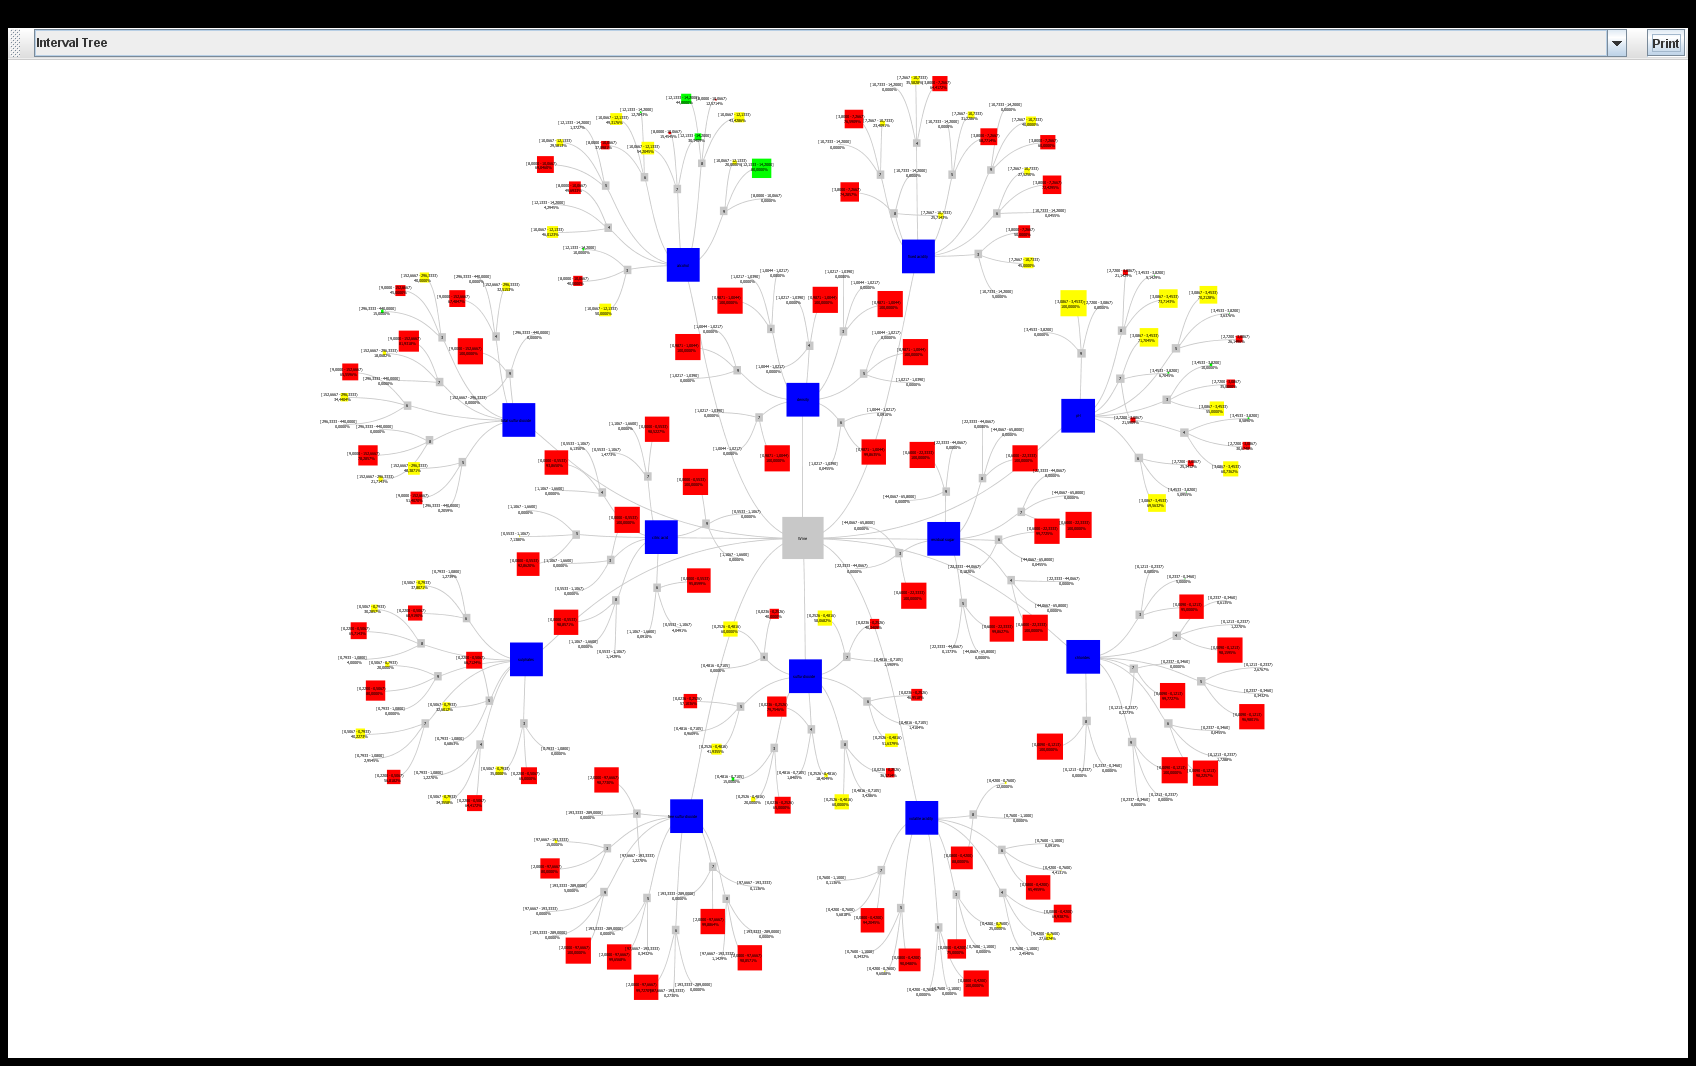
\includegraphics[width=\textwidth]{images/20131105033557plot.png}
  \caption{Overview with the Interval Tree}
  \label{oit}
\end{figure}


\begin{figure}[!h]
  \centering
  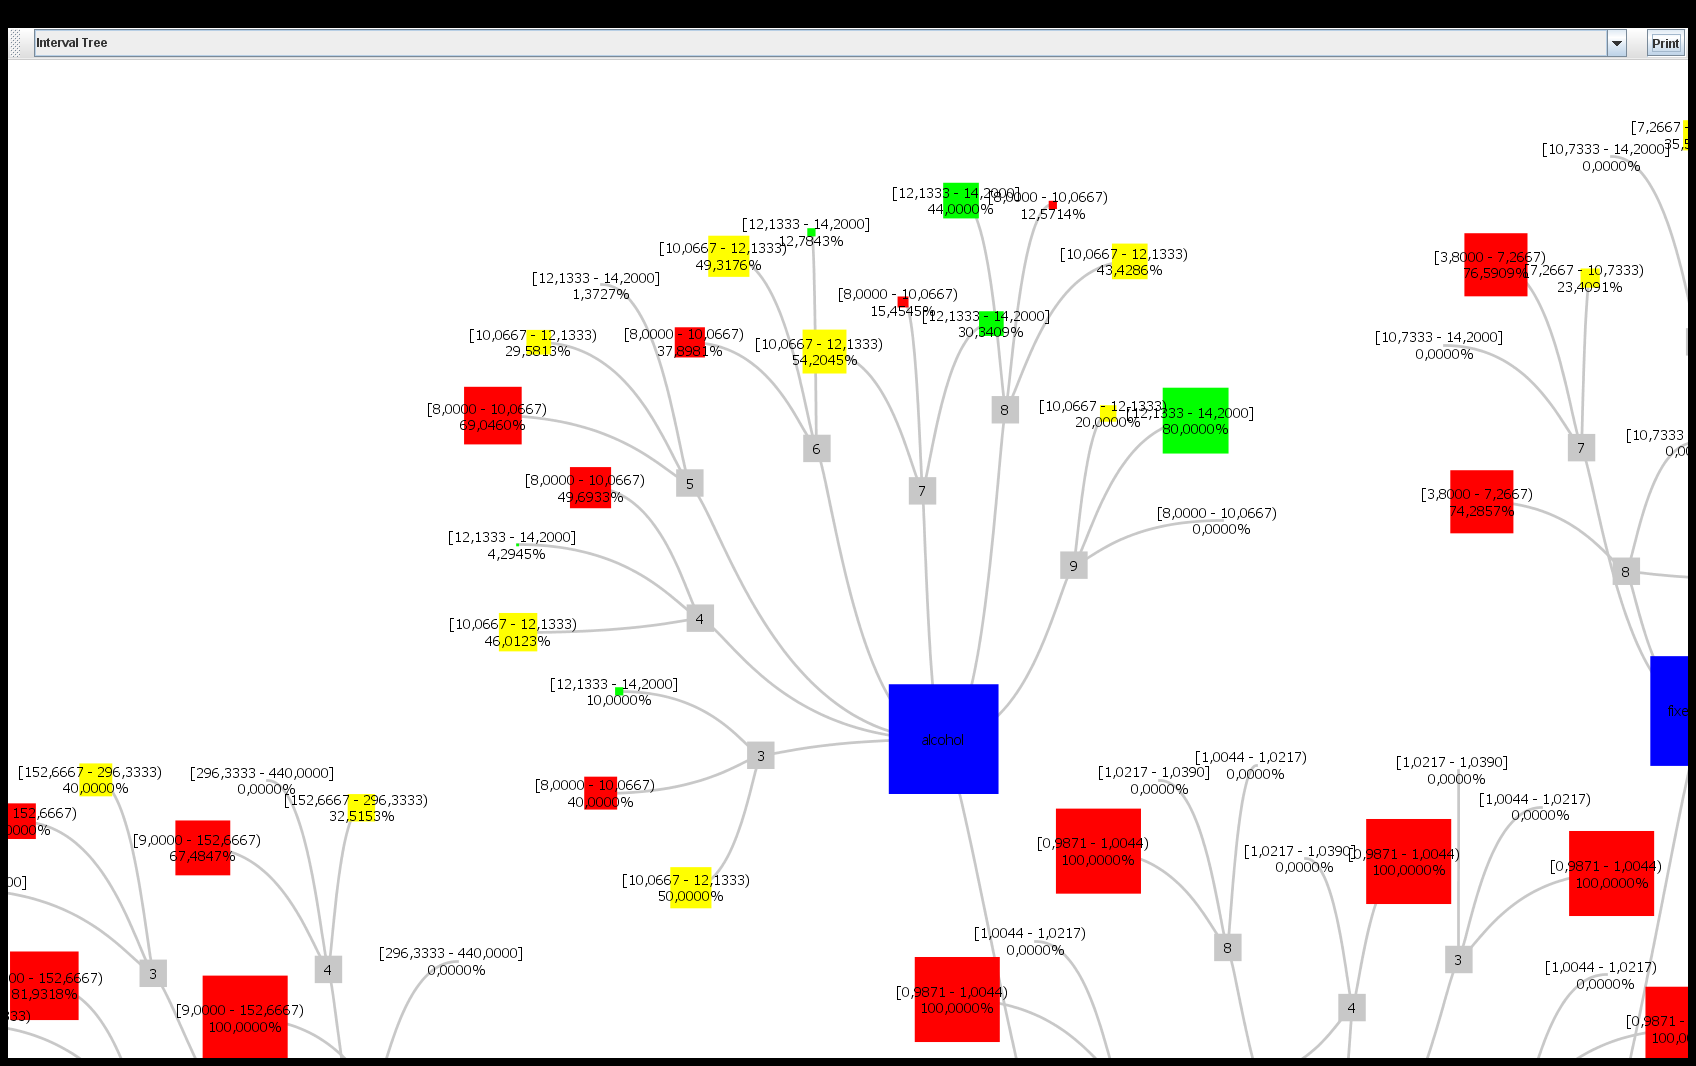
\includegraphics[width=\textwidth]{images/20131105034138plot.png}
  \caption{The alcohol branche in more detail}
  \label{ait}
\end{figure}

As can be seen, a graph like the interval tree does not always give nice results. As can be seen when looking at the density as shown in figure \ref{rsit}. Even when the number of intervals is increased to 5, we still get a very unbalanced result, which makes the interval tree clearly useless for the analysis of the densisty.

\begin{figure}[!h]
  \centering
  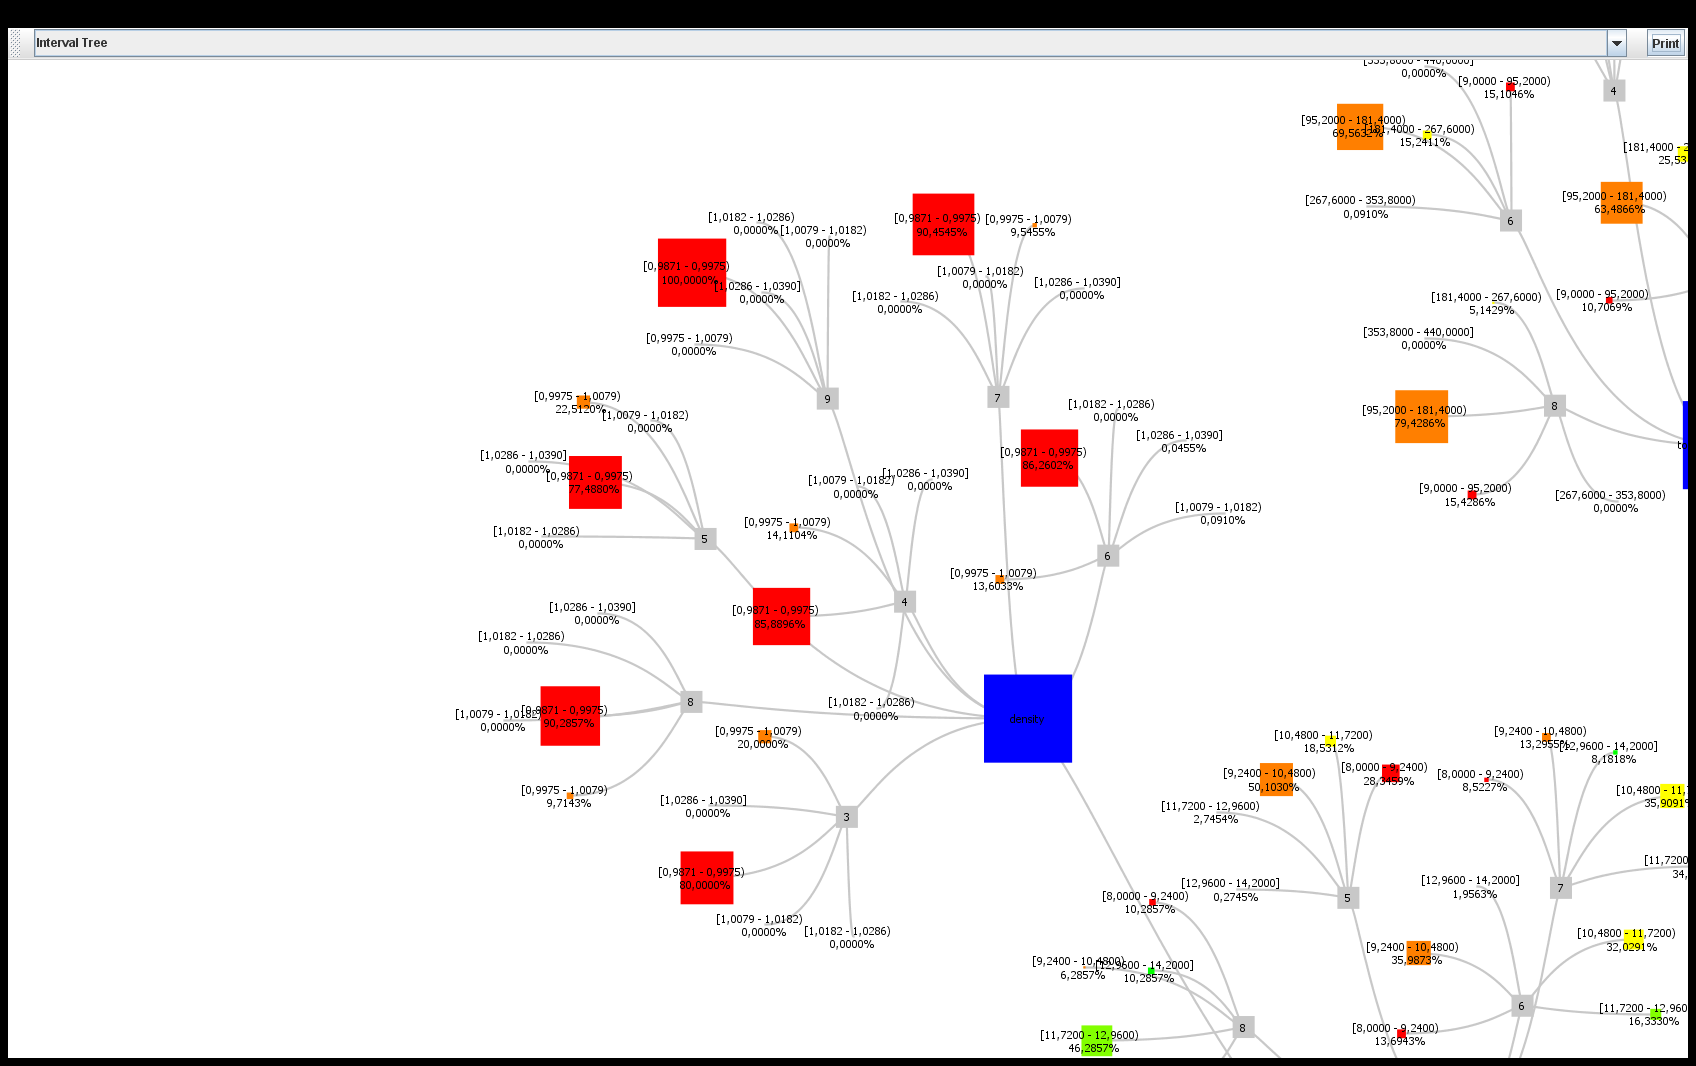
\includegraphics[width=\textwidth]{images/20131105041005plot.png}
  \caption{The density branch in more detail in the Interval Tree}
  \label{rsit}
\end{figure}

When using the average tree however, the results are much better as can be seen in figure \ref{rsmt}, we can now clearly see that a lower density is better then a high density.

\begin{figure}[!h]
  \centering
  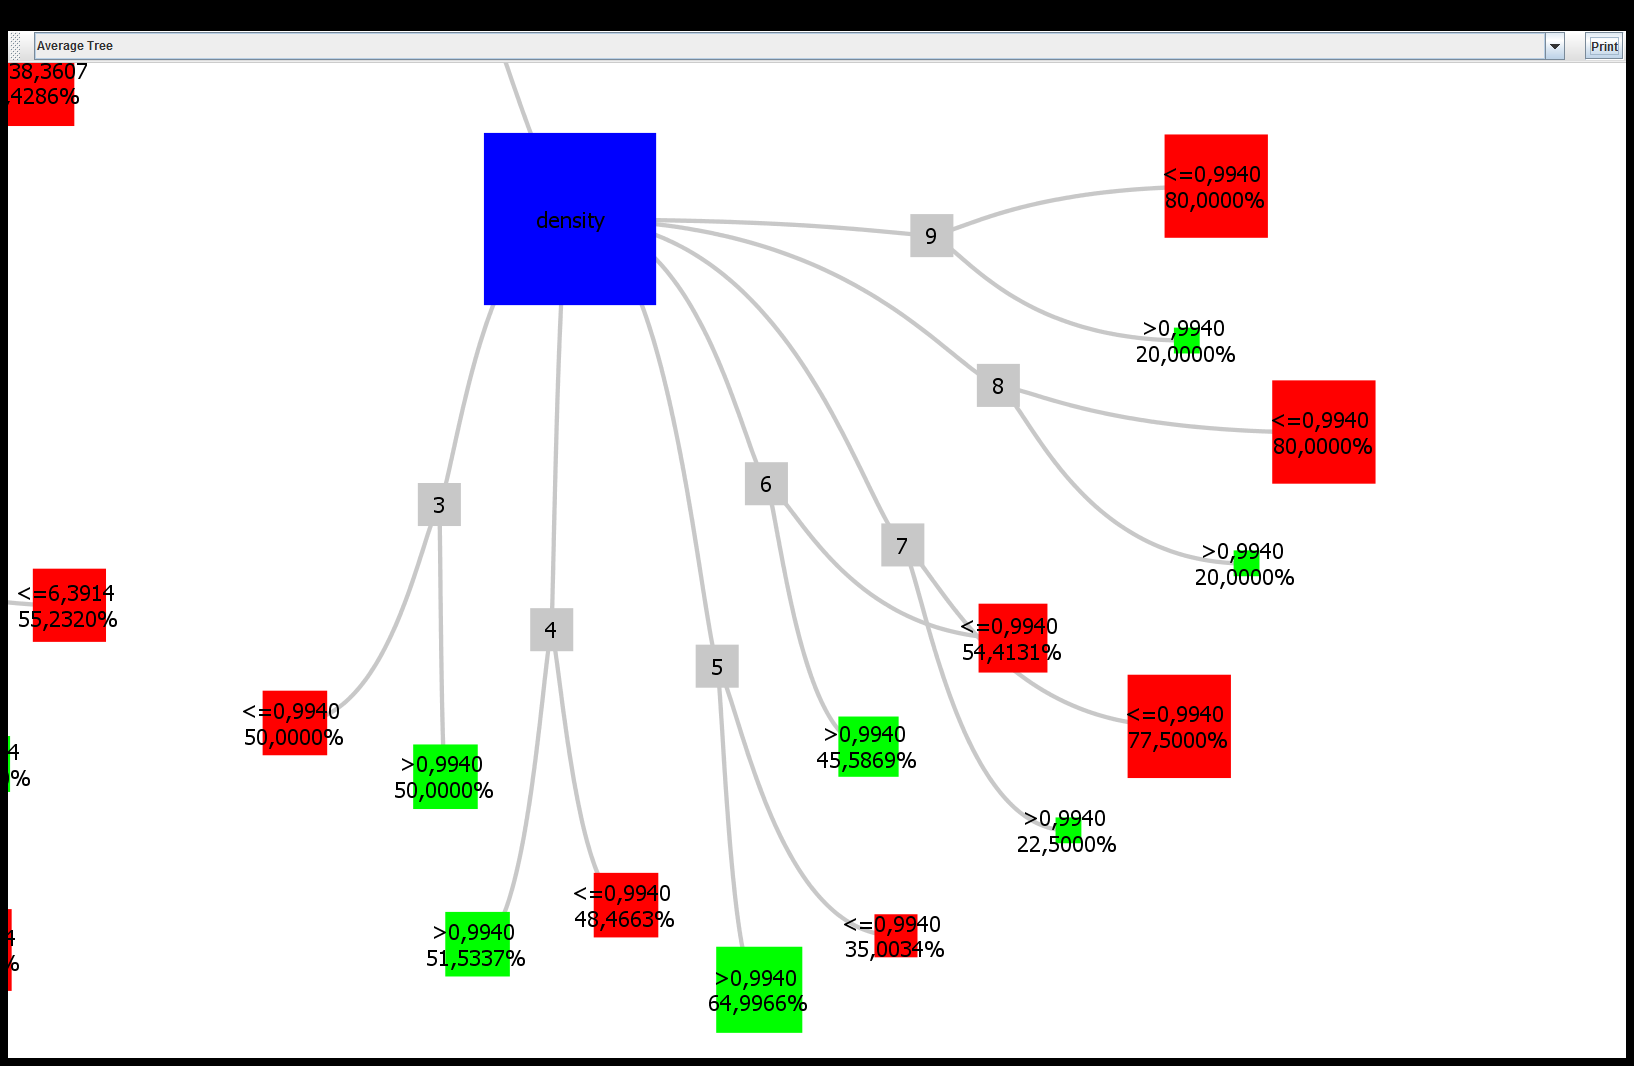
\includegraphics[width=\textwidth]{images/AverageTree.png}
  \caption{The density branch in more detail in the average tree}
  \label{rsmt}
\end{figure}

\section{Conclusion}
For the analysis we could clearly see that our application works, although it is not always helpfull in finding the actual answers we are looking for, multiple visualizations have to be used in order to branch down to the actual answer. We tried to add a feature to the program so that it would be able to link the visualizations together, but did not manage to get this to work properly. We expect that if this worked, we could much easier see the correlation between the datapoints and what actually makes a good wine. Since we could start eliminating unhelpfull parameters, while keeping more valuable one included. \\

However, we did manage to produce visualizations which actually helped determining what makes a high quality wine, which is a (relatively) high alcohol and sulfur dioxide concentration while the concentration of chlorides and total and residual sulfur dioxide is low.

\end{document}
